% !TeX encoding = ISO-8859-2

\chapter{Gerinc �s borda az emberi testben}

\begin{wrapfigure}{l}{0.4\textwidth}
	\begin{center}
		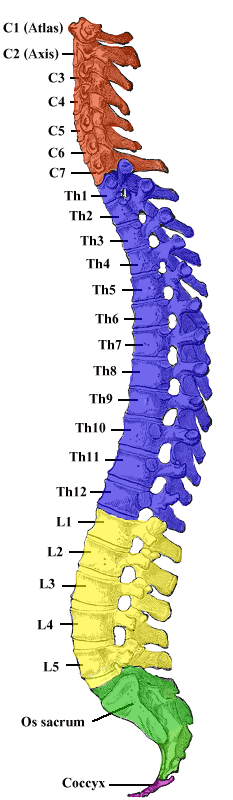
\includegraphics[width=0.3\textwidth]{gerinc}
	\end{center}
	\caption{Emberi gerincoszlop} \label{fig:gerinc}
\end{wrapfigure}

Az embernek norm�lis esetben 33 gerinccsigoly�ja van.
A fels� 24 porckorongokkal van elv�lasztva egym�st�l.
Az als� 9 �ssze van n�ve.
Az csigoly�kat k�l�nb�z� r�gi�kra oszthatjuk elhelyezked�s�k szerint.
Az embernek az els� 7 csigoly�ja a nyaki, a k�vetkez� 12 a h�ti, az ut�na k�vetkezik 5 �gy�ki, ezt�n j�n 5 keresztcsonti �s v�g�l 4 farokcsonti.
Minden csigoly�nak megvan a saj�t sorssz�ma, mely \aref{fig:gerinc} �br�n l�that�.


%\lipsum[1]

%\todoi{H�ny bord�ja, csigoly�ja van t�bbnyire egy embernek stb...}